\section{Introduction}

\subsection{Contexte}
\begin{frame}[c]{Contexte}
	\begin{itemize}
		\item Utilité de la jurisprudence pour les juristes
		\begin{itemize}
			\item elle est analysée pour comprendre l'application de la loi
		\end{itemize}
	    \item Motivation : limite de l'analyse manuelle
	    \begin{enumerate}
	    	\item Gros volume de décisions 
	    		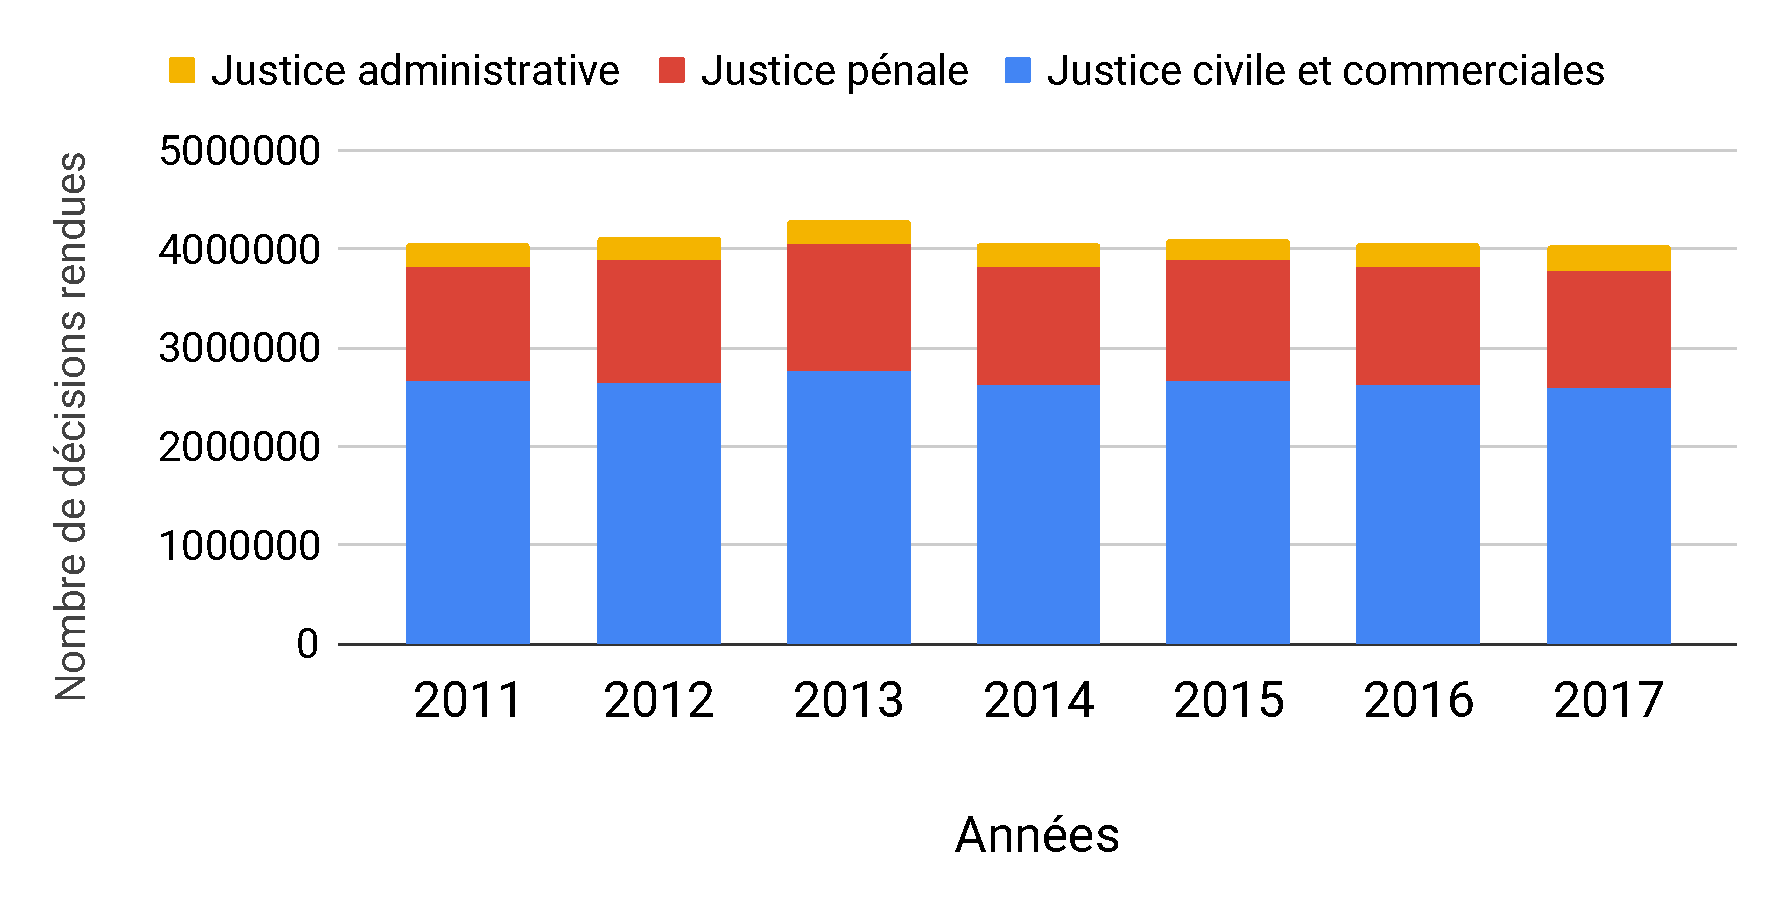
\includegraphics[width=0.6\textwidth]{chiffres-justice.pdf}   	
			\item Limite des moteurs de recherche juridique : 
			\begin{itemize}
				\item Pas de critère de recherche sémantique (catégorie de demande, type de faits, etc.)
				\item pas d'analyse synthétique de corpus
			\end{itemize}
	    \end{enumerate}
	\end{itemize}
\end{frame}

%\begin{frame}[c]{Motivation: gros volume de décisions}
%	\textbf{Plus de 4 millions de décisions prononcées / an}
%	\begin{figure}
%		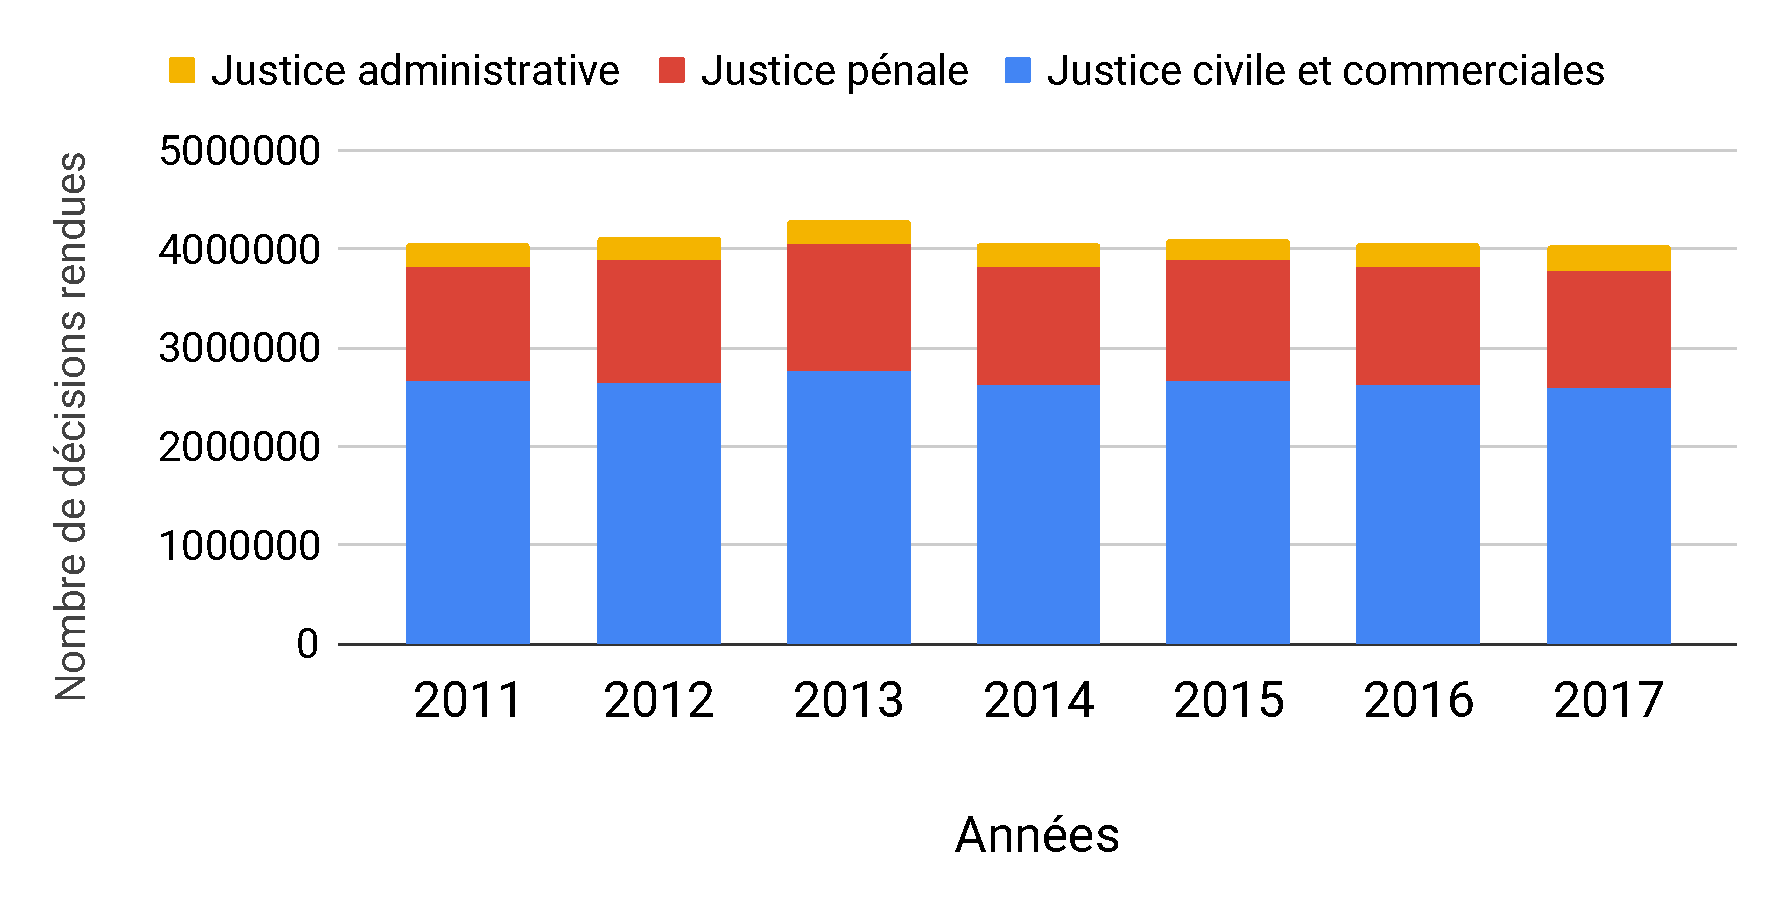
\includegraphics[width=\textwidth]{chiffres-justice.pdf}
%		\textit{\tiny{\textbf{Source}: \url{http://www.justice.gouv.fr/statistiques-10054/chiffres-cles-de-la-justice-10303/}}}
%		\caption{Nombre de décisions prononcées en France par an de 2011 à 2017.}
%	\end{figure}		
%\end{frame}
%
%\begin{frame}[t]{Motivation: recherches et analyses sémantiques difficiles}
%	
%	Moteurs de recherche juridique à mots-clés 
%	
%	Aucune analyse synthétique des décisions 
%	
%	\begin{figure}
%		\centering
%		\fbox{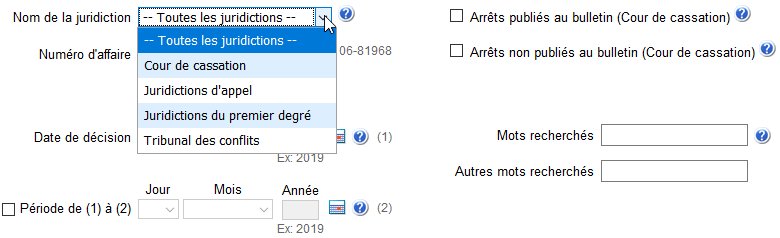
\includegraphics[width=0.9\textwidth]{legifrance.PNG}}
%		\caption{Formulaire de Légifrance.}
%	\end{figure}
%\end{frame}

\subsection{État de l'art}
\begin{frame}[c]{Activités en analyse automatique de décisions judiciaires}
	\scriptsize
	\begin{itemize}
		\item Extraction d'information dans les décisions
		\begin{itemize}  \scriptsize
			\item entités juridiques \cite{Waltl2016lexia, andrew2018legalNerAndRelation}
			\item faits \cite{wyner2010extractlegalelts, wyner2010casefactors, Shulayeva2017recognfactprincip}
			\item définitions de concept juridiques \cite{Waltl2016lexia,waltl2017legaliegerman}
			\item arguments \cite{moens2007NBvsMaxent4arguments}
		\end{itemize}
		\item Classification de décisions
		\begin{itemize} \scriptsize
			\item Prédiction des décisions de justice \cite{Ashley2009classifCases, Aletras2016predictDecisionECHR}
			\item identification de la formation et la période \cite{Sulea2017predictareadecision,sulea2017legalEnsSVM}
			\item identifier la sentence prononcée (Chine) \cite{ma2018wmdchinesecase}
		\end{itemize}
		\item Similarité entre décisions 
		\begin{itemize}  \scriptsize
			\item décisions qui citent les mêmes lois et précédents \cite{nair2018judgsimassorule}
			\item recherche d'affaires antérieures pertinentes  \cite{thenmozhi2017legalprecedretriev}
			\item identifier la sentence prononcée (Chine) \cite{ma2018wmdchinesecase}
			\item similarité basée sur la question discutée et les faits sous-jacents (Inde) \cite{kumar2011judgmentsimilarity}
			\item regroupement non-supervisé \cite{raghuveer2012legalclusteringLDA}
		\end{itemize}
	\end{itemize}
\end{frame}

\subsection{Objectif de la thèse}
\begin{frame}[c]{Objectif de la thèse}
	\begin{figure}[!htb]	
		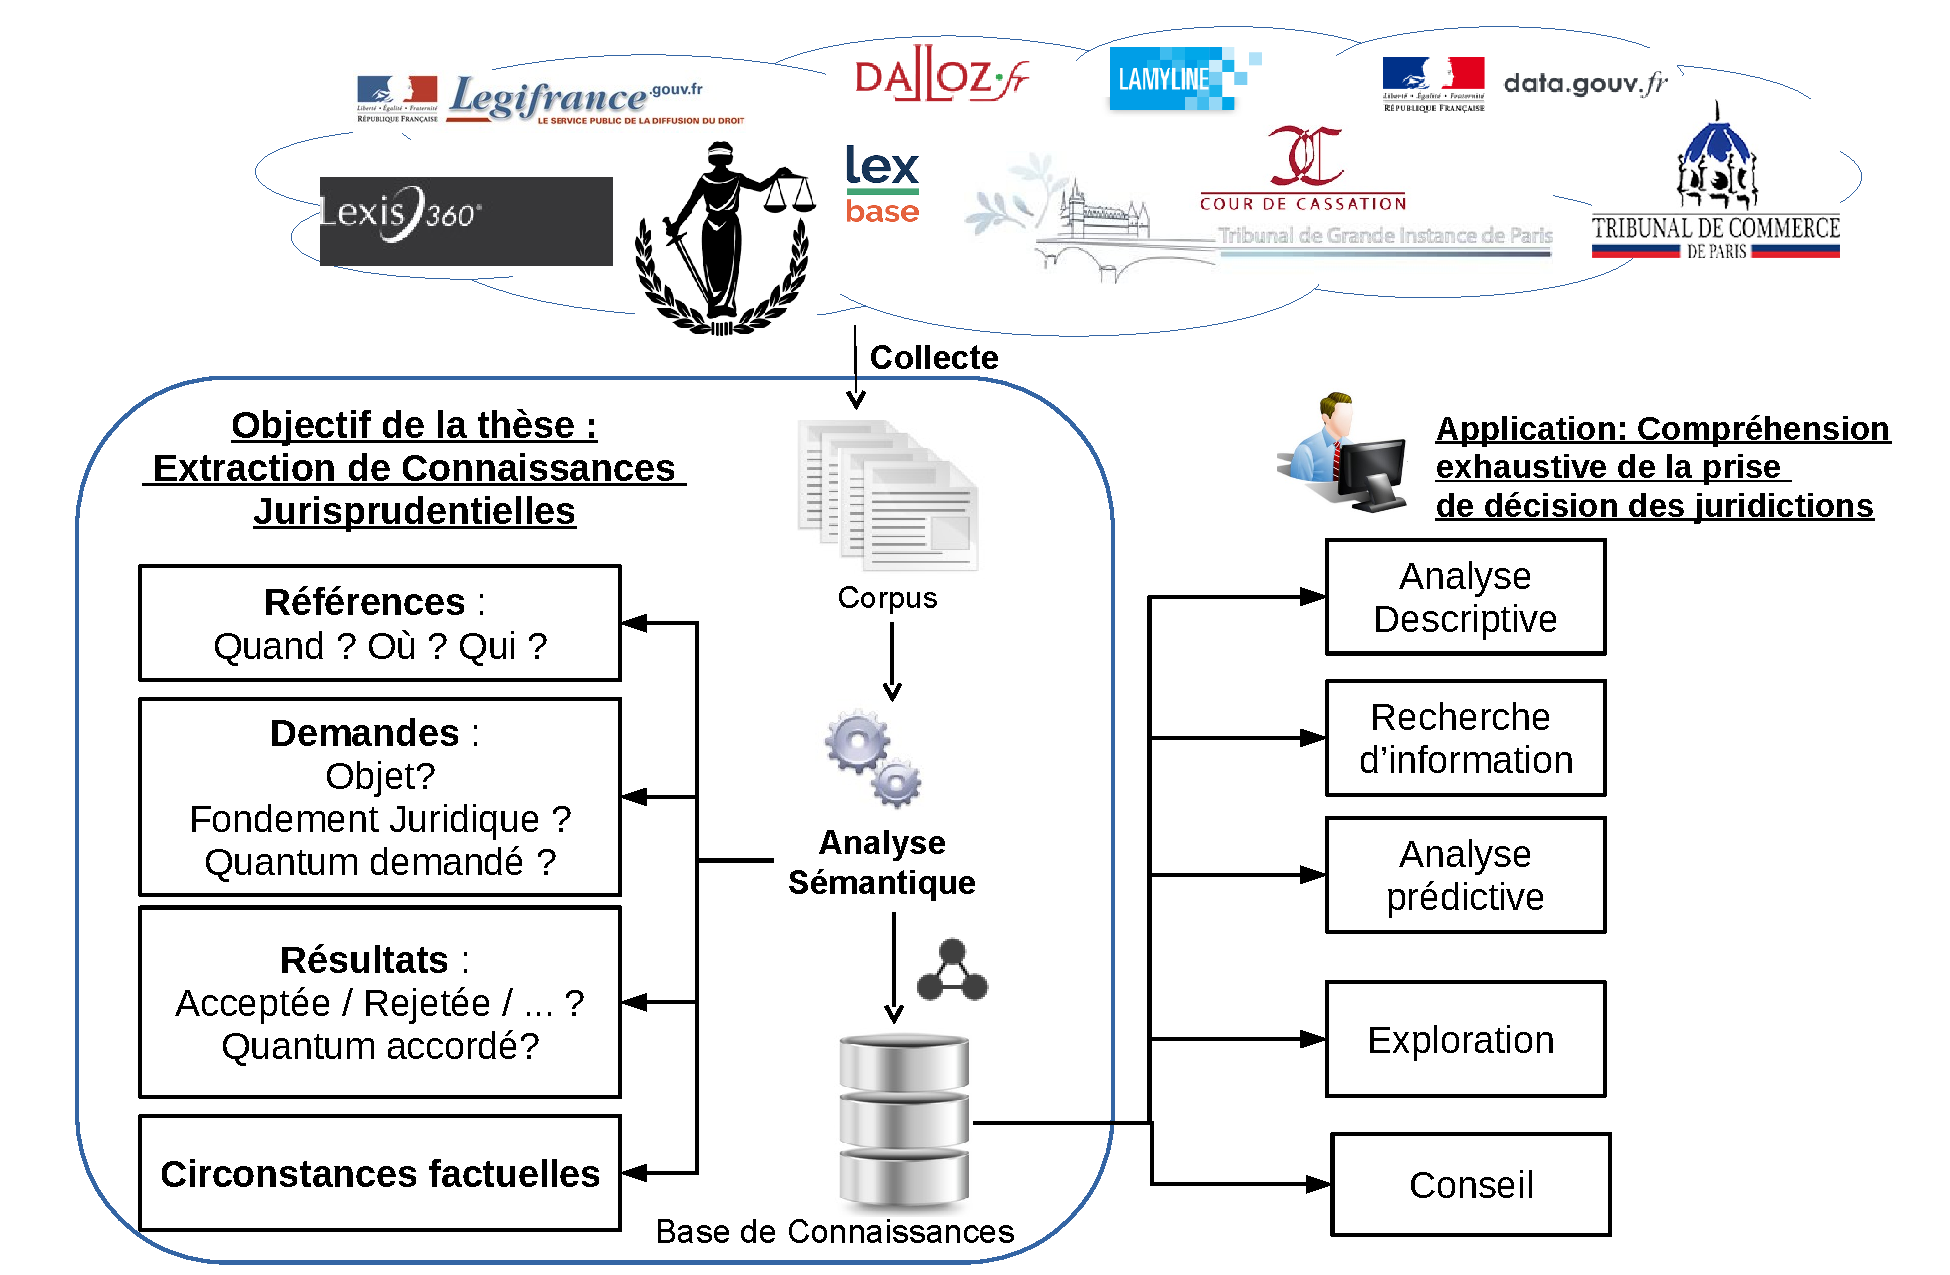
\includegraphics[width=\textwidth]{Objectif_these.pdf}
		\caption{Objectifs et exemples d'application de la thèse.} \label{fig:intro:objectif-these}
	\end{figure}
\end{frame}

\begin{frame}[c]{Problème : annotation de sections, méta-données, normes}
\begin{figure}
	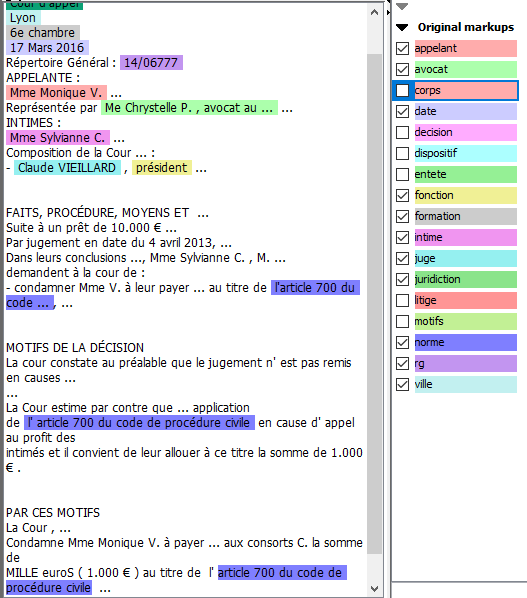
\includegraphics[height=\textheight]{decision-marquee.png}
\end{figure}
\end{frame}

\begin{frame}[c]{Problème : extraction des demandes}
	Cibles : sens du résultat, montant demandé, montant accordé
\begin{exampleblock}{Expression de demande et resultat}
%danais/CASAI1401082.xml
\scriptsize
Jennifer M. et Catherine M. ... demandent à la Cour de :

- \textcolor{orange}{infirmer le dit jugement} en \textcolor{blue}{toutes ses dispositions} ; 
...

Statuant à nouveau ...

- les condamner au paiement d' une somme de  \textbf{3 000,00 € pour procédure abusive} et
aux entiers dépens ; ...

La cour ...  

CONFIRME \textcolor{orange}{le jugement entrepris} en \textcolor{blue}{toutes ses dispositions}.

\end{exampleblock}

\scriptsize{\textit{Légende:  \textcolor{orange}{référence au jugement antérieur},  \textcolor{blue}{agrégation}}}


\begin{table} 
\centering 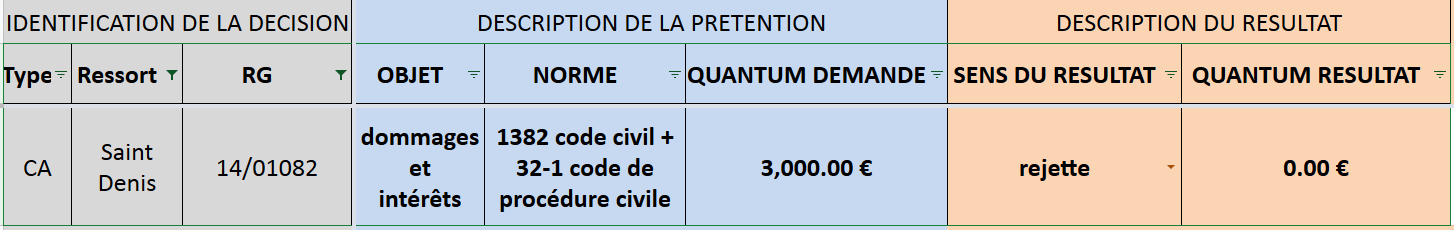
\includegraphics[width=\textwidth]{tab-danais.png}
\caption{\scriptsize Informations à extraire (dommages-intérêts pour procédure abusive)}
\end{table}
\end{frame}



\begin{frame}[c]{Positionnement en fouille de texte}	
	\begin{figure}[!htb]
		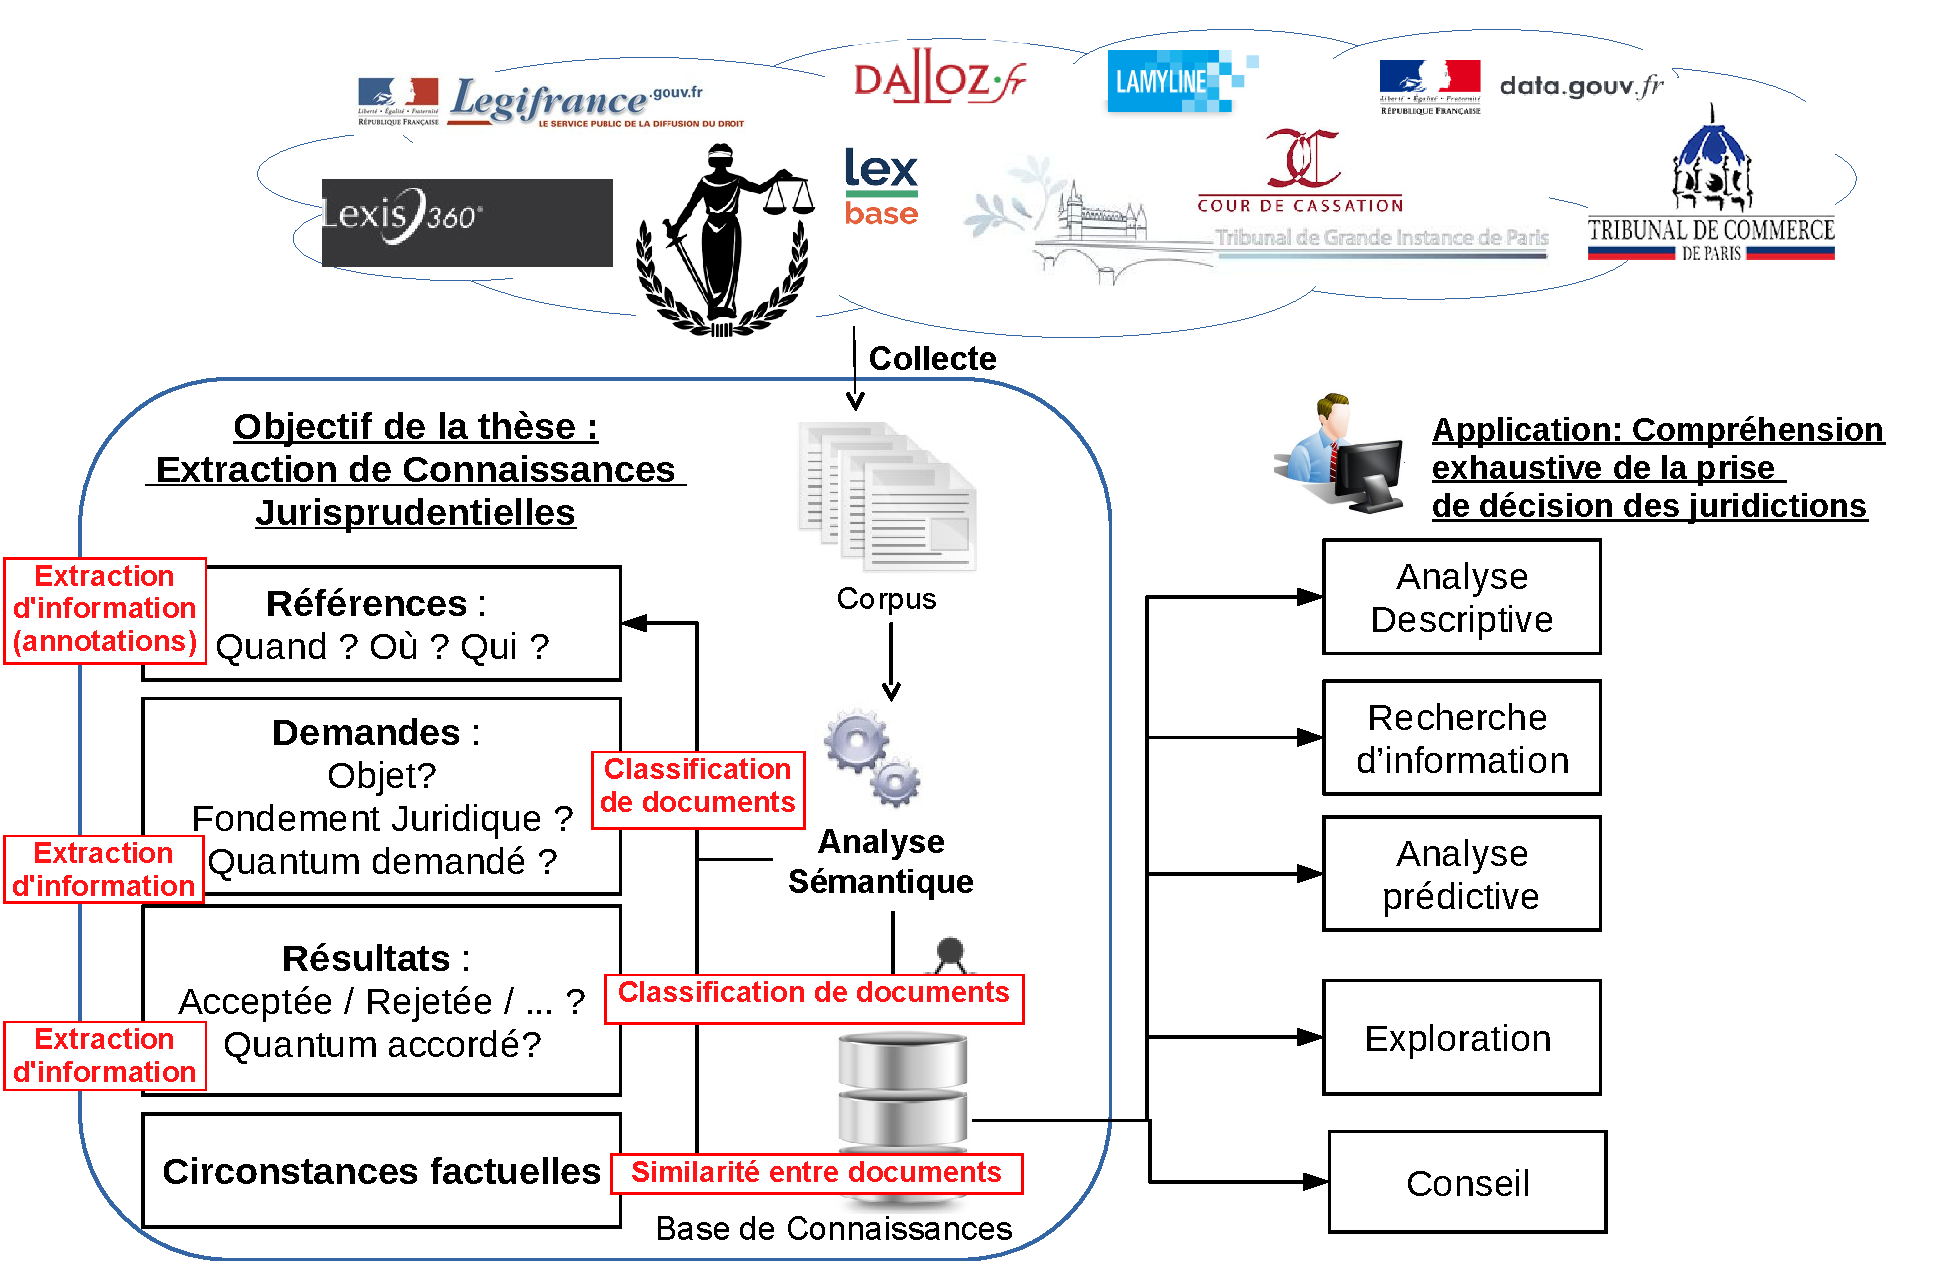
\includegraphics[width=\textwidth]{Objectif_these-problemes2.pdf}
		\caption{Tâches abordées en analyse de données textuelles.} \label{fig:intro:objectif-these-problemes}
	\end{figure}
\end{frame}

\begin{frame}{Difficultés rencontrées par l'automatisation de ces tâches}
	\begin{itemize}
		\item Les décisions sont des textes non-structurés
		\item Le langage juridique est complexe
	\end{itemize}	

	\tiny	
	\begin{columns}
		\begin{column}{.50\linewidth}
			ARRÊT N°
			
			R.G: 11/03924
			
			...
			
			{COUR D'APPEL} DE {NÎMES}
			
			{CHAMBRE CIVILE}
			
			{1ère Chambre A}
			
			ARRÊT DU {20 MARS 2012}
			
			APPELANTE:
			
			{Madame Michéle A.} ...
			
			assistée de la {SELARL VAJOU}, ...
			
			INTIMES:
			
			{Monsieur Martial B} ...
			
			assisté de la {SCP MARION GUIZARD PATRICIA SERVAIS}, ...
			
			COMPOSITION DE LA COUR LORS DU DÉLIBÉRÉ:
			
			{M. Dominique BRUZY, Président}
			
			{M. Serge BERTHET, Conseiller}
			
			...
		\end{column}
		\begin{column}{.50\linewidth}
			FAITS, PROCEDURE, ...
			
			Madame Michèle A. demande:
			
			...
			
			- de condamner Madame JONES-B. à lui payer la somme de {2.500 euros} au titre de l'{article 700 du Code de Procédure Civile}, 
			
			\vspace{0.4cm}
			
			PAR CES MOTIFS, LA COUR:
			
			...
			
			Vu l'{article 809 du Code de Procédure Civile},
			
			...
			
			{Déboute Madame A. de sa demande de provision sur dommages-intérêts.}
			
			...
			
			Vu l'{article 700 du Code de Procédure Civile},
			
			Condamne Madame JONES-B. à verser à Madame A. la somme de {2.500 euros}.
		\end{column}
	\end{columns}
\end{frame}